\chapter{Projekcije in zmanjšanje dimenzionalnosti podatkov}

Modeli, ki jih gradimo v strojnem učenju, povzemajo podatke tako, da v nekem formalnem zapisu predstavijo glavne vzorce, ki so te podatke oblikovali. V primeru večdimenzionalnih podatkov nas tako na primer zanima, ali bi podatke lahko popisali z manjšim številom spremenljivk. Z izborom značilk smo se ukvarjali že v prejšnjem poglavju, a nas bo tu zanimalo, če lahko podatke predstavimo z novimi značilkami, ki bi podatke lahko predstavili bolj kompaktno, pri tem odkrili kakšno zanimivo preslikavo starih v nove značilke, ter morda celo dosegli, da je novih značilk izjemno malo. Recimo, dve, tako da lahko vse primere izrišemo v razsevnem diagramu in tam s pomočjo vizualizacije razmišljamo o njihovih podobnosti in strukturi prostora primerov. Ljudje smo vizualna bitja in nam izris kart primerov lahko intuitivno pove več kot pa recimo matematične enačbe, ki morda te povezujejo.

Začnimo s primerom. Na sliki~\ref{f:torbice} so ženske torbice različnih proizvajalcev. Z uporabo že zgrajenih globokih mrež za razvrščanje slik lahko slike torbic pretvorimo v vektorje. Mreža Inception v3 nam na svojem predzadnjem nivoju na primer za vsako sliko vrne vektor dolžine 2048, oziroma sliko popiše z 2048 atributi. S postopki, ki jih bomo opisali v tem poglavju, lahko take opise zmanjšamo in predstavimo torbice v nizko dimenzionalnem prostoru. Slika~\ref{f:torbice-mds} tako prikazuje predstavitev primerov v dvodimenzionalnem prostoru, kjer je razvidno, da ena Hermesova torbica bolj podobna torbicam ostalih proizvajalcev, in da se je Dior pri eni od torbic zgledoval po torbicah Chanela. Morda. Vsekakor bi ta opažanja morali preveriti, a je zanimivo, kako hitro nas vizualizacije navdahnejo z idejami. Prav zato so vizualizacije v odkrivanju znanj iz podatkov tako pomembne in zato so pomembne tudi tehnike zmanjšanja dimenzionalnosti in odkrivanja nizko dimenzionalnih projekcij podatkov.

\begin{figure}[htbp]
\centering{
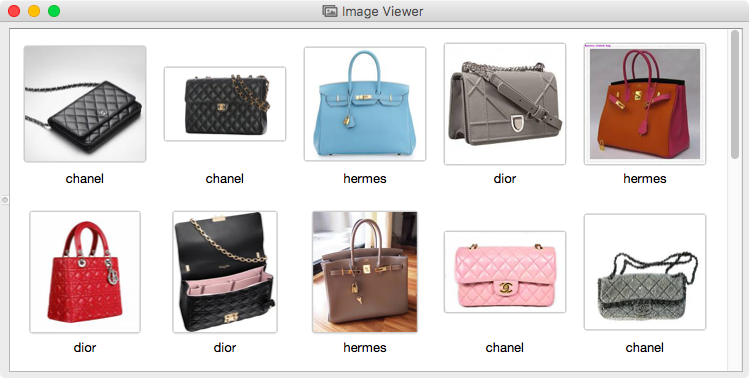
\includegraphics[width=12cm]{slike/torbice.png}
\caption{Ženske torbice različnih proizvajalcev.}
\label{f:torbice}}
\end{figure}

\begin{figure}[htbp]
\centering{
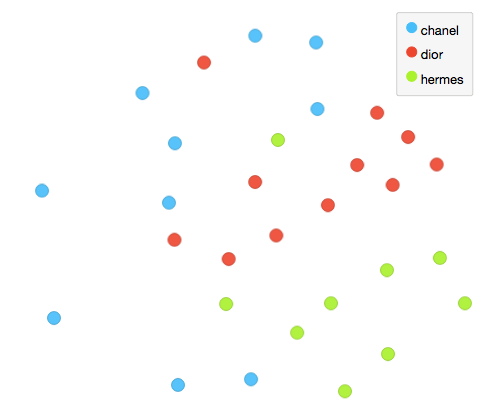
\includegraphics[width=8cm]{slike/torbice-mds.png}
\caption{Predstavitev ženskih torbic s slike~\ref{f:torbice} v dvodimenzionalnem prostoru.}
\label{f:torbice-mds}}
\end{figure}

\section{Metoda glavnih komponent}

Prva, morda tudi najbolj znana metoda za zmanjšanje dimenzij in odkrivanje zanimivih projekcij podatkov je metoda glavnih komponent. Predpostavimo, da imamo dano matriko učnih primerov $X\in\mathbb{R}^{m\times n}$, kjer je $m$ število primerov in $n$ število atributov. Primer $x^{(i)}\in X$, torej $i$-ti primer v učni množici primerov, bo tako opisan z $n$ atributi $x\in\mathbb{R}^{n}$, za katere bomo tu privzeli, da so njihove vrednosti realna števila. V splošnem iščemo projekcije podatkov tako, da atributni zapis primerov z $n$ atributi nadomestimo z atributnim zapisom z $k$ novimi atributi tako, da je $k\ll n$ in da nam novi atributi povedo čim več o primerih iz učne množice.

Pričnimo s $k=1$, torej s projekcijo v eno samo dimenzijo. Dogovorimo se, da bo naša projekcija linearna in da bomo vrednost novega atributa tvorili kot linearno kombinacijo originalnih atributov. Smer projekcijske ravnine oziroma smer premice, na katero bomo projicirali podatke označimo z enotskim vektorjem $u_1$, za katerega torej velja $u_1^\tr u_1=1$.

Naj bo $x^{(i)}$ primer iz učne množice. Njegova projekcija na projekcijsko ravnino je skalar, $u_1 x^{(i)}\in \mathbb{R}$. Naj bo $\bar{x}$ središčna točka podatkov:
%
$$ \mean{x}=\frac{1}{m}\sum_i x^{(i)}$$
%
Projekcija središčne točke na projekcijsko ravnino je $u_1 \mean{x}$. Primeri v učni množici odstopajo od središčne točke, eni bolj, drugi manj. Primere bi želeli projicirati na ravnino tako, da ta odstopanja čim bolj zajamemo, torej, da so tudi v projicirani ravnini čim večja. Povprečno kvadratno odstopanje v projekciji od projekcije središčne točke imenujemo tudi varianca točk v projekciji:
%
$$ \Var(u_1^\tr X^\tr)=\frac{1}{n}\sum_{i=1}^m \big(u_1^\tr x^{(i)}-u_1^\tr\mean{x}\big)^2 $$

Z drugimi besedami, želimo poiskati tak projekcijski vektor $u_1$, ki maksimizira varianco projekcije $\Var(u_1^\tr X^\tr)$. Poigrajmo se malce z enačbo za varianco projekcije:
%
\begin{equation}
  \begin{split}
    \Var(u_1^\tr X^\tr)
    & = \frac{1}{m}\sum_{i=1}^m \big(u_1^\tr x^{(i)}-u_1^\tr\mean{x}\big)^2 \\
    & = \frac{1}{m}\sum_{i=1}^m \big(u_1^\tr x^{(i)} u_1^\tr x^{(i)} - 2 u_1^\tr x^{(i)} u_1^\tr \mean{x} + u_1^\tr \mean{x} u_1^\tr \mean{x} \big)
  \end{split}
\end{equation}
%
Tu upoštevamo, da je $u_1^\tr x$ skalarni produkt dveh vektorjev, in da je transponirana vrednost realnega števila enaka temu številu. Torej je na primer $u_1^\tr x=(u_1^\tr x)^\tr=x^\tr u_1$. Z upoštevanjem tega se nam zgornji izraz primerno poenostavi:
%
\begin{equation}
  \begin{split}
    \Var(u_1^\intercal X^\tr)
    & = \frac{1}{m}\sum_{i=1}^m u_1^\tr \big(x^{(i)} {x^{(i)}}^\tr - 2 x^{(i)} \mean{x}^\tr + \mean{x}~\mean{x}^\tr \big) u_1 \\
    & = u_1^\tr \big( \frac{1}{m}\sum_{i=1}^m (x^{(i)}-\mean{x}) (x^{(i)}-\mean{x})^\tr\big) u_1
  \end{split}
\end{equation}

V oklepaju je kovariančna matrika! Prejšnji stavek smo končali s klicajem zato, ker je kovarianca znan in mnogokrat uporabljan koncept v statistiki in nam pove, kako sta dve naključni spremenljivki povezani. Označimo kovariančno matriko s ${\rm S}$:
\begin{equation}
  {\rm S} = \frac{1}{m}\sum_{i=1}^m (x^{(i)}-\mean{x}) (x^{(i)}-\mean{x})^\tr
\end{equation}

V našem primeru imamo $n$ atributov, kar pomeni, da je kovariančna matrika dimenzije ${\rm S}=\mathbb{R}^{n\times n}$. Zapišimo še enkrat dobljeno enačbo za varianco:
\begin{equation}
  \Var(u_1^\intercal X^\tr) = u_1^\tr {\rm S} u_1
\end{equation}
%
Spomnimo, da je naš namen poiskati projekcijski vektor $u_1$ pri katerem je zgornja varianca maksimalna. Za vektor $u_1$ zahtevamo, da je to enotni vektor (sicer maksimizacija zgornje enačbe ne bi imela smisla, saj bi to dosegli z neskončno dolgim vektorjem $u_1$). Maksimizacijo variance, kjer iščemo ustrezen vektor $u_1$ z omejitvijo $u_1^\tr u_1=1$ rešimo z uporabimo Lagrangeovih multiplikatorjev. Maksimiziramo torej izraz:
%
\begin{equation}
  f(u_1) = u_1^\tr {\rm S} u_1 + \lambda_1(1-u_1^\tr u_1)
\end{equation}
%
V maksimumu bo odvod zgornje enačbe enak nič:
\begin{equation}
  \frac{\partial f(u_1)}{\partial u_1}={\rm S} u_1 - \lambda_1 u_1=0
\end{equation}
%
kar pomeni,
\begin{equation}
  {\rm S} u_1=\lambda_1 u_1
\end{equation}
%
Tu je ${\rm S}$ matrika katere vrednosti poznamo, $u_1$ je vektor, ki ga iščemo, $\lambda_1$ pa skalar. Poznano? Seveda! Zgornjemu pogoju ustreza le tak $u_1$, ki je lastni vektor matrike ${\rm S}$. Ampak korelacijska matrika ima več lastnih vektorjev. Kateri med njimi je pravi? Množimo zgornjo enačbo z $u_1^\tr$:
%
\begin{equation}
  u_1^\tr {\rm S} u_1 = u_1^\tr \lambda_1 u_1=\lambda_1 u_1^\tr u_1=\lambda_1
\end{equation}
%
Na levi je izraz za našo varianco $\Var(u_1^\intercal X^\tr)$, ki jo skušamo maksimizirati. Vemo, da mora biti $u_1$ lastni vektor kovariančne matrike. Skladno z zgornjo enačbo pa sedaj tudi vemo, da je to lastni vektor z najvišjo pripadajočo lastno vrednostjo.

V smeri vektorja $u_1$ se lega naših primerov $X$ v $n$-dimenzionalnem prostoru torej najbolj spreminja, njihova varianca je v tej smeri največja. Z $u_1^\tr X^\tr$ dobimo pravokotno projekcijo vsakega od primerov na to os. S to projekcijo, oziroma legi v smeri $u_1$, smo pojasnili največjo varianco primerov. Kaj še ostane? Vse, kar je pravokotno na smer $u_1$. Največjo varianco na pravokotni hiperravnini pa je ravno v smeri drugega lastnega vektorja, saj je ta pravokoten na $u_1$, to je vektorja, ki ima drugo največjo lastno vrednost. Pojasnjen delež te variance je $\lambda_2$, skupaj pa s pravokotno projekcijo na prvi in drugi lastni vektor pojasnimo $\lambda_1+\lambda_2$ variance množice primerov.

Lastni vektorji kovariančne matrike nam določajo nov koordinatni
sistem, kjer so koordinate, po vrsti, tiste, po katerih se lege točk v
večdimenzionalnem prostoru najbolj spreminjajo, oziroma je njihova
varianca največja. Nove koordinate, urejene skladno z lastnimi vrednostmi vektorjev, imenujemo komponente primerov v novem, transformiranem sistemu. Ker nas bodo zanimale samo te z visokimi deleži razložene variance jih bomo imenovali {\em glavne komponente}.

\begin{figure}[htbp]
\centering{
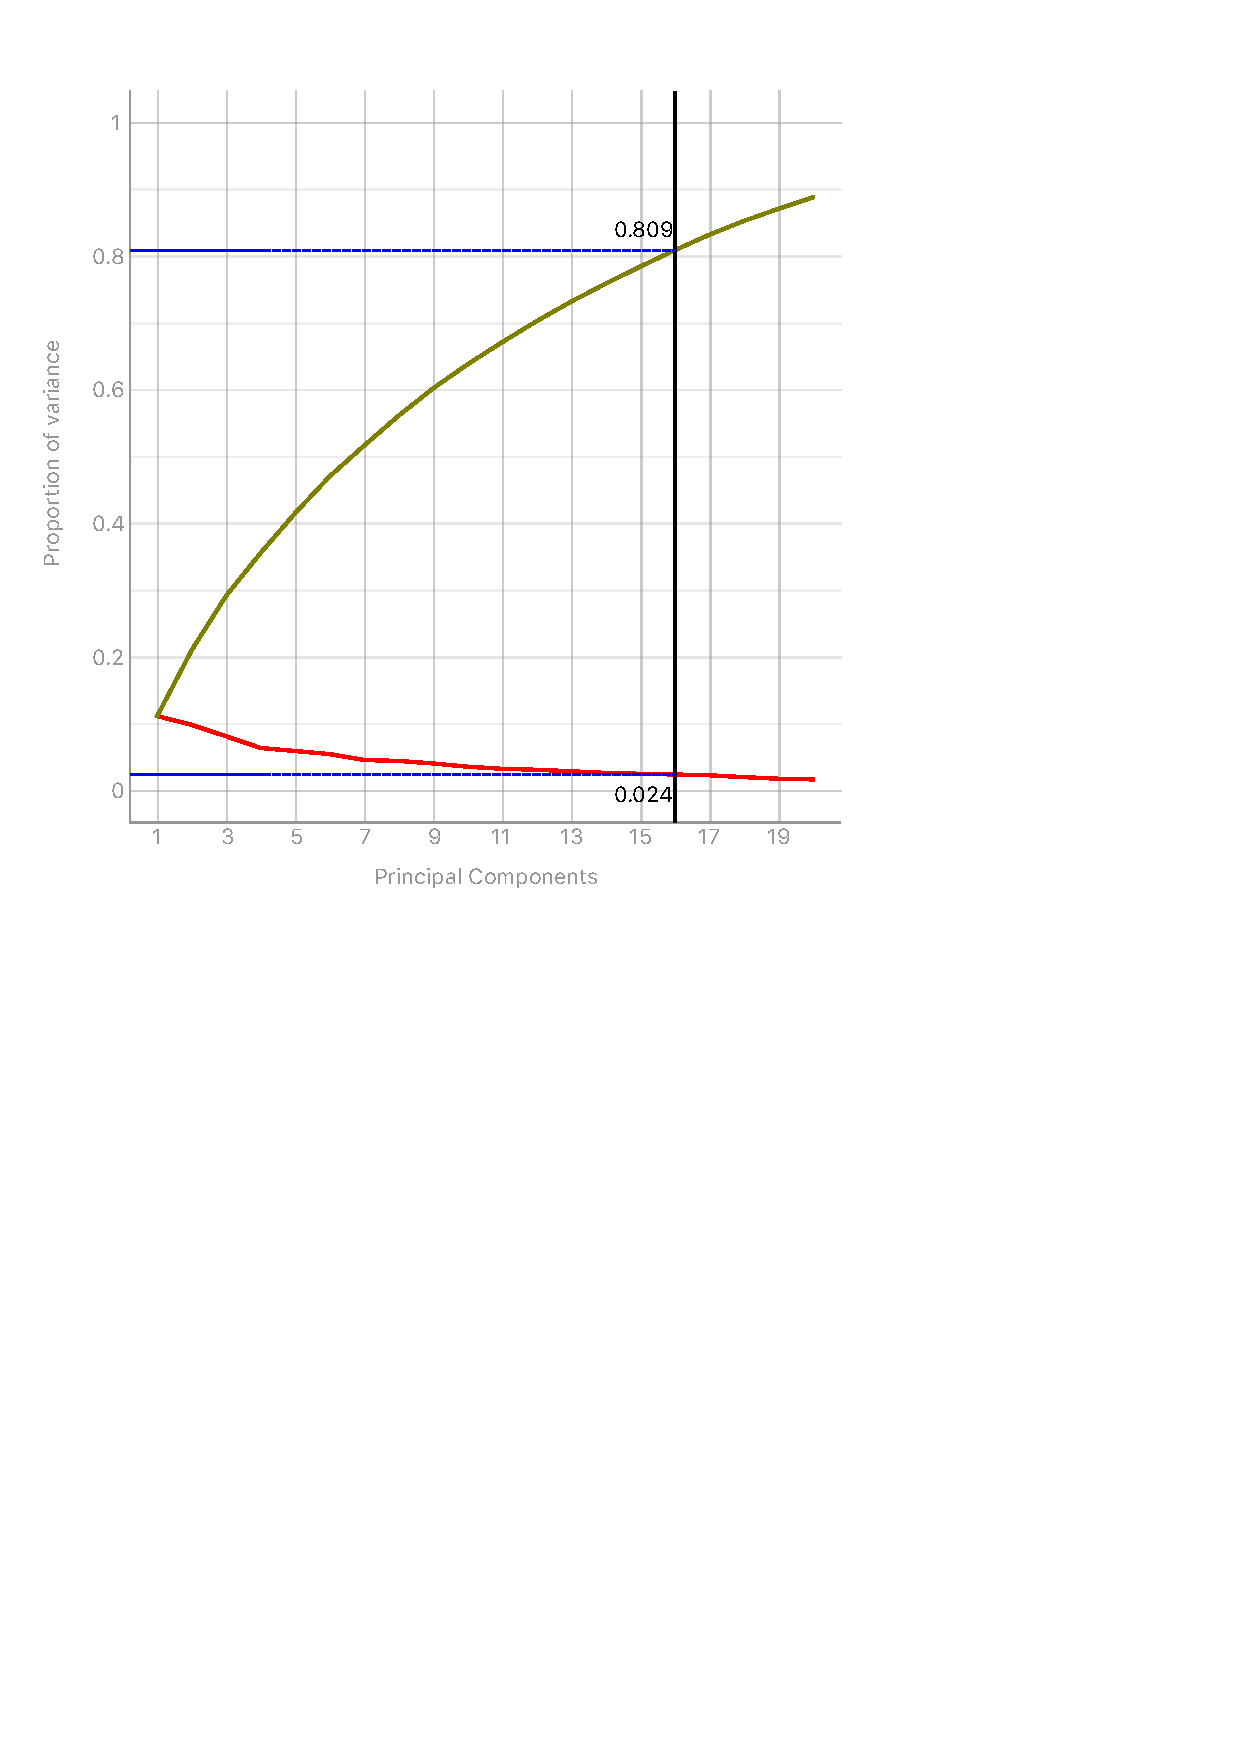
\includegraphics[width=8cm]{slike/scree-diagram.pdf}
\caption{Graf odvisnosti razložene variance od števila glavnih komponent (zgornja črta) za podatke o torbicah iz slike~\ref{f:torbice}.}
\label{f:scree}}
\end{figure}

V splošnem nas zanima, koliko najvišje rangiranih dimenzij v novem
koordinatnem sistemu zares potrebujemo za opis podatkov. Pri tem moramo
seveda določiti, kakšen je naš ciljni delež pojasnjene variance. Tipično
smo zadovoljni, če izbrano število komponent pojasni vsaj $80\%$ skupne variance. Ker skupno varianco poznamo (enaka je vsoti kvadratov razdalj do
centra), je potrebno torej le določiti, koliko začetnih urejenih lastnih
vrednosti moramo sešteti, da njihova vsota predstavlja želeni delež razložene variance. Primer grafa, ki kaže odvisno deleža razložene variance glede na število glavnih komponent kaže slika~\ref{f:scree}.

Pristop glavnih komponent se mnogokrat uporablja tudi samo za namene vizualizacije, kjer primere, opisane z mnogimi atributi, želimo predstaviti v dvodimenzionalni ravnini. Pri tem se moramo seveda zavedati, da prvi dve komponenti razložijo morda le majhen del celotne variance.

Za konec, naj ponovimo. Za predstavitev podatkov z glavnimi komponentami je potrebno podatke najprej osrediščiti in nato poiskati kovariančno matriko. Lastni vektorji kovariančne matrike so bazni vektorji novega, transformiranega sistema, njihove lastne vrednosti pa povedo, kakšen delež variance nam razloži posamezna komponenta.

\section{Računski postopki določanja glavnih komponent}

Še praktičen razmislek: v primerih velikega števila atributov bo računanje vseh lastnih vektorjev in vrednosti zamudno. Še posebej, če nas zanima samo projekcija podatkov v dvodimenzionalni prostor. Prvi lastni vektor kovariančne matrike $M$ lahko rajši (hitreje) določimo numerično, s potenčno metodo. Vzamemo nek naključni vektor (npr. $x$), ga transformiramo z matriko $M$ (torej, izračunamo $x\leftarrow M x$), in to ponavljamo do konvergence. Ob vsakem koraku tako dobljeni $x$ normaliziramo, torej, $x\leftarrow \frac{M x}{\norm{M x}}$. Na ta način dobimo lastni vektor. Kako izračunamo pripadajočo lastno vrednost?
\begin{equation}
  M u = \lambda u
\end{equation}

\begin{equation}
  u^\tr M u = u^\tr \lambda u = \lambda u^\tr u = \lambda
\end{equation}

Kako določimo naslednjo komponento? Ena od možnosti je, da uporabimo ravnokar izračunani lastni vektor, nanj projiciramo podatke, te vrednosti odštejemo od podatkov (torej dobimo projekcijo na lastnemu vektorju pravokotno hiperravnino) in za te podatke ponovno izračunamo kovariančno matriko ter s potenčno metodo njej lastni vektor z največjo lastno vrednostjo. V primeru, da potrebujemo več komponent, postopek ustrezno ponovimo.

Za primer, ko nas zanima samo projekcija podatkov v ravnino lahko potenčno metodo namesto na vektorju izvedemo na sistemu dveh vektorjev $U$. Vektorja matrike $U$ morata biti pravokotna. To dosežemo tako, da po vsakem koraku potenčne metode uporabimo Gram-Schmidtovo ortogonalizacijo.

\endinput

\section{Singularni razcep}

Oglejmo si podatke šestih filmskih zanesenjakov in njihovih ocenah filmov v tabeli~\ref{t:romance-sf}. Že na prvi pogled lahko opazimo, da imam najbrž dve skupini ocenjevalcev in dve skupini filmov. Metka, Neža, Maja in Tina ne marajo znanstvene fantastike in jim je bolj blizu romantika. Alojz in Gašper pa rajši gledata znanstveno fantastiko in jima romantični filmi niso prav blizu.

\begin{table}
\begin{tabular}{rcccccc}
\toprule
 & Cvetje & Titanic & Harry & Sally & Alien & Prometheus \\
\midrule
Metka & 1 & 2 & 1 & 0 & 0 \\
Neža & 2 & 4 & 2 & 0 & 0 \\
Maja & 3 & 5 & 3 & 0 & 0 \\
Tina & 5 & 10 & 5 & 0 & 0 \\
Alojz & 0 & 1 & 0 & 1 & 2 \\
Gašper & 0 & 0 & 0 & 2 & 4 \\
\bottomrule
\end{tabular}
\label{t:romance-sf}
\end{table}

Skupine pa nismo našli samo pri ocenjevalcih. Že zgoraj smo filme razvrstili v dve skupini, in te uganili iz kratkih nazivov filmov. Pa lahko te skupine, torej skupine uporabnikov in skupine filmov, razpoznamo algoritmično? Lahko podatke, ki jih imamo zgoraj, predstavimo v neki zgoščeni obliki, kjer bi iz zgoščenega zapisa bilo možno prepoznati skupine in interakcijo med ocenjevalci in filmi. Opazimo, recimo, da vsaka od vrstic v naši ocenjevalni tabeli izvira od enega od spodnjih vrstičnih vektorjev, ki ga moramo ustrezno pomnožiti z neko konstanto. 
% 
$$
\begin{bmatrix}
1 & 1 & 1 & 0 & 0 \\
0 & 0 & 0 & 1 & 1 \\
\end{bmatrix}
$$
Lahko take vektorje prepoznamo iz podatkov? Tehnika, ki jo bomo za to uporabili, se imenuje {\em singularni razcep}. Podatki iz tabele~\ref{t:romance-sf} so že sicer zapisani v atributni obliki in jih lahko torej predstavimo v matriki $A=\mathbb{R}^{m\times n}$. To matriko v splošnem s singularnim razcepom zapišemo kot produkt treh matrik:
\begin{equation}
A = U\Sigma V^\tr
\end{equation}
kjer so:
\begin{itemize}
\item leva singularna matrika $U\\mathbb{R}^{m\times r}$, ki $m$ objektov v vrsticah predstavi v $r$-dimenzionalnem prostoru,
\item desna singularna matrika 
\end{itemize}

\cleardoublepage
